\chapter{วิธีการดำเนินการวิจัย}
\label{chapter:experiment}

% \section{วิธีการดำเนินการ}

% สำรวจข้อผิดพลาดของระบบเดิมที่พบเห็นอย่างละเอียด ตรวจสอบและรวบรวมความต้องการของผู้ใช้ สรุปความต้องการของผู้ใช้และออกแบบโครงสร้างและระบบของเว็บไซต์ ประชุมวางแผนงานดำเนินการตามแผนที่วางไว้ จากนั้นทำการ Deploy เพื่อให้ผู้ใช้งานได้ใช้งานจริง

\section{ความต้องการของระบบ}

\subsection{ระบบสามารถแสดงสถิติได้}

ระบบจะต้องสามารถแสดงสถิติการแข่งขันทุกครั้งที่ผ่านมาได้ โดยจะต้องสามารถดูสถิติการแข่งขันทดสอบทักษะการคิดเชิงคำนวณได้ทั้งระดับมัธยมต้นและมัธยมปลายของโรงเรียนของผู้ใช้งานได้และจะต้องสามารถแสดงสถิติการแข่งขันโดยรวมของโรงเรียนทั้งหมดได้

\subsection{ระบบจัดการรายชื่อของผู้สมัคร}

ระบบจะต้องสามารถเพิ่มข้อมูลของผู้ใช้ลงในฐานข้อมูลได้ ระบบจะต้องสามารถลบข้อมูลของผู้ใช้ออกจากฐานข้อมูลได้ ระบบจะต้องสามารถแก้ไขข้อมูลของผู้ใช้ได้

\section{การวิเคราะห์และออกแบบระบบ}
\subsection{ภาพรวมของระบบ}

\begin{figure}[ht]
    \centering
    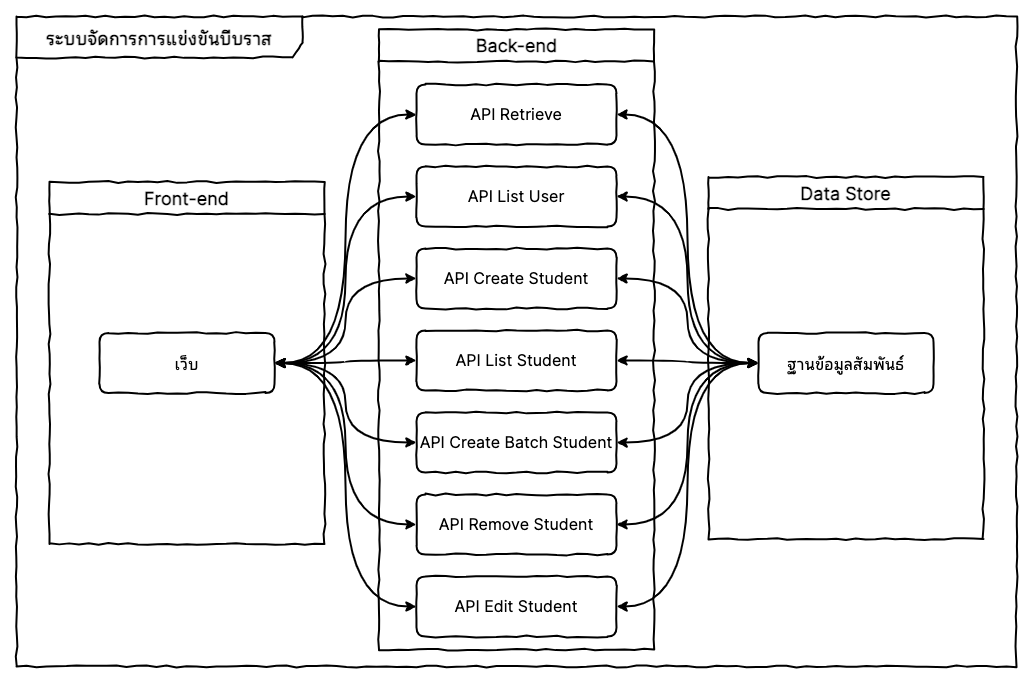
\includegraphics[width=120mm,scale=1.0]{diagrams/system-overview-diagram.png}
    \caption{ภาพรวมของระบบอย่างง่าย}
    \label{fig:system-overview-diagram}
\end{figure}

\subsection{แผนภาพแสดงการทำงานของผู้ใช้ระบบ (Use Case Diagram)}

\begin{figure}[ht]
    \centering
    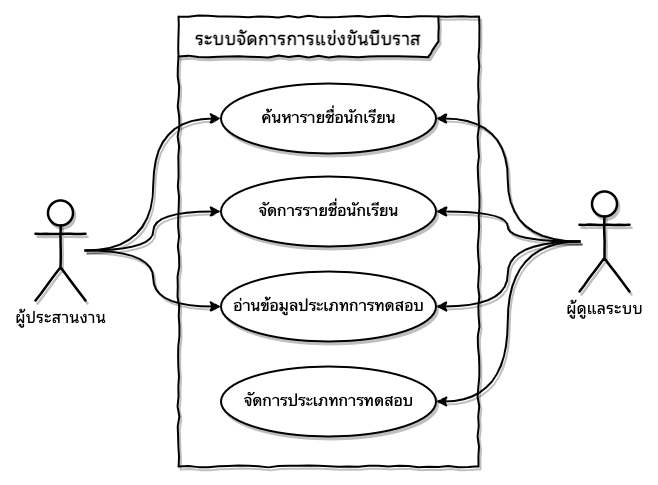
\includegraphics[width=120mm,scale=1.0]{diagrams/use-case-diagram.png}
    \caption{แผนภาพแสดงการทำงานของผู้ใช้ระบบจัดการแข่งขันบีบราส}
    \label{fig:use-case-diagram}
\end{figure}
\subsection{คำอธิบายของระบบ}

ระบบแสดงสถิติและจัดการรายชื่อของผู้สมัครแข่งขันทดสอบทักษะการคิดเชิงคำนวณแบ่งออกเป็น 2 ส่วน ได้แก่

\begin{enumerate}
    \item \textbf{ส่วนแสดงสถิติการแข่งขัน} ผู้ใช้สามารถเลือกที่การ์ดการแข่งขัน (Contest) เพื่อให้แสดงข้อมูลการแข่งขันได้โดยเบื้องต้นระบบจะแสดงเป็นข้อมูลสถิติการแข่งขันทั้งหมดและข้อมูลสถิติการแข่งขันของโรงเรียนของผู้ใช้งาน โดยผู้ใช้สามารถเลือกที่จะค้นหา (Search) สถิติการแข่งขันของแต่ละโรงเรียนหรือแต่ละบุคคลได้เมื่อทำการค้นหาระบบจะแสดงข้อมูลสถิติตามการค้นหานั้น
    \item \textbf{จัดการรายชื่อของผู้สมัครแข่งขัน} ในกรณีที่ผู้ใช้งานคือผู้ดูแลระบบ (Admin) สามารถเลือกที่การ์ดครู (Teacher) ในกรณีที่ผู้ใช้งานเป็นผู้ประสานงาน (Coordinator) สามารถเลือกที่การ์ดนักเรียน (Student) เพื่อจัดการกับรายชื่อนักเรียนได้
\end{enumerate}

\section{โครงสร้างฐานข้อมูลในระบบ (Database Schema)}

\begin{figure}[ht]
    \centering
    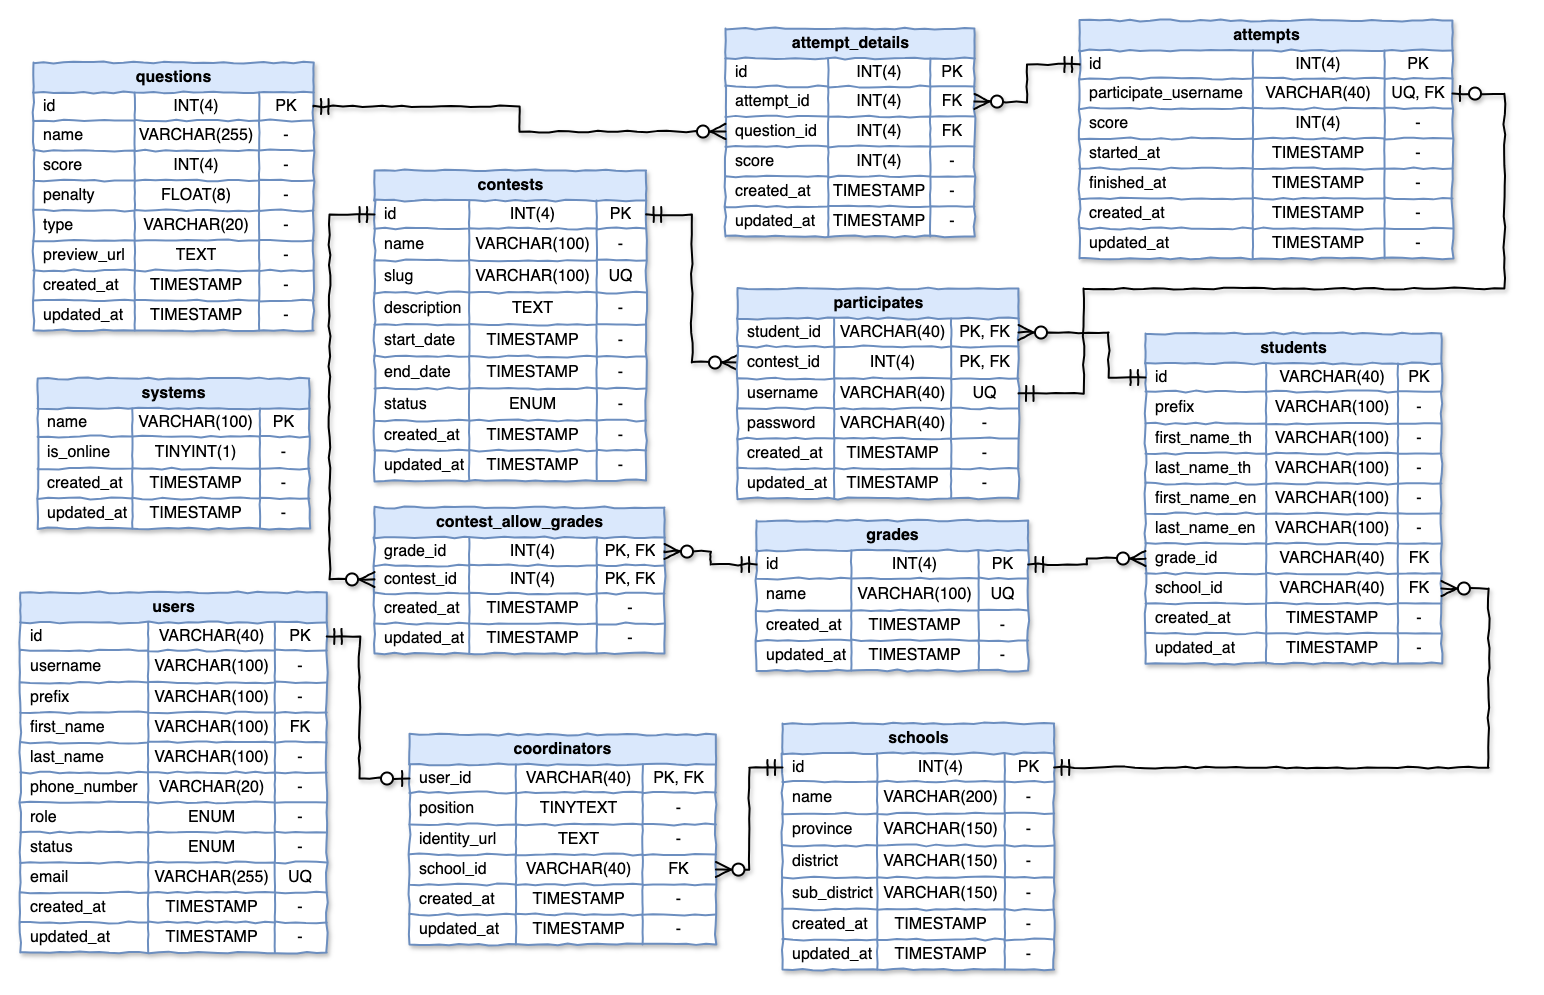
\includegraphics[width=120mm,scale=1.0]{diagrams/database.png}
    \caption{แผนภาพข้อมูลระดับโครงสร้างของฐานข้อมูลในระบบ}
    \label{fig:physical-database-diagram}
\end{figure}

\section{พจนานุกรมข้อมูล (Data Dictionary)}

\subsection{ตารางข้อมูลในระบบ}
\begin{table}[H]
    \caption{ตารางข้อมูลในระบบ พร้อมคำอธิบาย}
    \label{tab:database}
    \begin{tabularx}{\textwidth}{ | p{3cm} | X | }
    \hline
    \textbf{ชื่อตาราง} & \textbf{คำอธิบาย} \\
    \hline
    contests & จัดเก็บประเภทการแข่งขัน \\
    \hline
    grades & จัดเก็บระดับชั้นของนักเรียน \\
    \hline
    schools & จัดเก็บข้อมูลโรงเรียนในประเทศไทย \\
    \hline
    students & จัดเก็บข้อมูลของนักเรียนที่สมัครเข้าแข่งขัน \\
    \hline
    systems & จัดเก็บสถานะการเปิด-ปิดของระบบ \\
    \hline
    users & จัดเก็บข้อมูลส่วนตัวของผู้ใช้ \\
    \hline
    user\_coordinators & จัดเก็บข้อมูลของผู้ใช้ที่เป็นผู้ประสานงานเพื่อยืนยันตัวตน \\
    \hline
    \end{tabularx}
\end{table}
    

\subsection{พจนานุกรมข้อมูลของตาราง}
\begin{table}[H]
    \caption{พจนานุกรมข้อมูลของตาราง contests}
    \label{tab:database-contests}
    \begin{tabularx}{\textwidth}{ | p{2.25cm} | p{2.20cm} | p{2.45cm} | p{2cm} | X | }
    \hline
    \textbf{ชื่อข้อมูล} & \textbf{ประเภทข้อมูล} & \textbf{ขนาดของข้อมูล} & \textbf{ข้อจำกัด} & \textbf{คำอธิบาย} \\
    \hline
    id & int & 4 & primary\_key & รหัสการแข่งขัน \\
    \hline
    name & VARCHAR & 100 & required & ชื่อการแข่งขัน \\
    \hline
    slug & VARCHAR & 100 & required & รอแก้ \\
    \hline
    description & TEXT & 2 - 64Kb & - & คำอธิบายการแข่งขัน \\
    \hline
    start\_date & TIMESTAMP & 4 & required & เวลาที่เริ่มการแข่งขัน \\
    \hline
    end\_date & TIMESTAMP & 4 & required & เวลาที่สิ้นสุดการแข่งขัน \\
    \hline
    status & ENUM & 1 & required  & เวลาที่เริ่มการแข่งขัน \\
    \hline
    created\_at & TIMESTAMP & 4 & - & เวลาที่สร้างข้อมูล \\
    \hline
    updated\_at & TIMESTAMP & 4 & - & เวลาที่แก้ไขข้อมูลล่าสุด \\
    \hline
    \end{tabularx}
\end{table}

\begin{table}[htbp]
    \caption{พจนานุกรมข้อมูลของตาราง grades}
    \label{tab:database-grades}
    \begin{tabularx}{\textwidth}{ | p{2.25cm} | p{2.20cm} | p{2.45cm} | p{2cm} | X | }
    \hline
    \textbf{ชื่อข้อมูล} & \textbf{ประเภทข้อมูล} & \textbf{ขนาดของข้อมูล} & \textbf{ข้อจำกัด} & \textbf{คำอธิบาย} \\
    \hline
    id & VARCHAR & 40 & primary\_key & รหัสระดับชั้น \\
    \hline
    name & VARCHAR & 100 & required & ชื่อระดับชั้น \\
    \hline
    created\_at & TIMESTAMP & 4 & - & เวลาที่สร้างข้อมูล \\
    \hline
    updated\_at & TIMESTAMP & 4 & - & เวลาที่แก้ไขข้อมูลล่าสุด \\
    \hline
    \end{tabularx}
\end{table}

\begin{table}[H]
    \caption{พจนานุกรมข้อมูลของตาราง schools}
    \label{tab:database-schools}
    \begin{tabularx}{\textwidth}{ | p{2.25cm} | p{2.20cm} | p{2.45cm} | p{2.15cm} | X | }
    \hline
    \textbf{ชื่อข้อมูล} & \textbf{ประเภทข้อมูล} & \textbf{ขนาดของข้อมูล} & \textbf{ข้อจำกัด} & \textbf{คำอธิบาย} \\
    \hline
    id & INT & 4 & primary\_key & รหัสโรงเรียน \\
    \hline
    name & VARCHAR & 200 & required & ชื่อโรงเรียน \\
    \hline
    province & VARCHAR & 150 & - & จังหวัด \\
    \hline
    district & VARCHAR & 150 & - & เขต/อำเภอ \\
    \hline
    sub\_district & VARCHAR & 150 & - & แขวง/ตำบล \\
    \hline
    created\_at & TIMESTAMP & 4 & - & เวลาที่สร้างข้อมูล \\
    \hline
    updated\_at & TIMESTAMP & 4 & - & เวลาที่แก้ไขข้อมูลล่าสุด \\
    \hline
    \end{tabularx}
\end{table}

\begin{table}[H]
    \caption{พจนานุกรมข้อมูลของตาราง students}
    \label{tab:database-students}
    \begin{tabularx}{\textwidth}{ | p{2.25cm} | p{2.20cm} | p{2.45cm} | p{2cm} | X | }
    \hline
    \textbf{ชื่อข้อมูล} & \textbf{ประเภทข้อมูล} & \textbf{ขนาดของข้อมูล} & \textbf{ข้อจำกัด} & \textbf{คำอธิบาย} \\
    \hline
    id & VARCHAR & 40 & primary\_key & รหัสนักเรียน \\
    \hline
    prefix & VARCHAR & 100 & required & คำนำหน้า \\
    \hline
    first\_name\_th & VARCHAR & 100 & required & ชื่อจริงภาษาไทย \\
    \hline
    last\_name\_th & VARCHAR & 100 & required & นามสกุลภาษาไทย \\
    \hline
    first\_name\_en & VARCHAR & 100 & required & ชื่อจริงภาษาอังกฤษ \\
    \hline
    last\_name\_en & VARCHAR & 100 & required & นามสกุลภาษาอังกฤษ \\
    \hline
    grade\_id & VARCHAR & 40 & foreign\_key & รหัสระดับชั้น \\
    \hline
    school\_id & VARCHAR & 40 & foreign\_key & รหัสโรงเรียน \\
    \hline
    created\_at & TIMESTAMP & 4 & - & เวลาที่สร้างข้อมูล \\
    \hline
    updated\_at & TIMESTAMP & 4 & - & เวลาที่แก้ไขข้อมูลล่าสุด \\
    \hline
    \end{tabularx}
\end{table}

\begin{table}[H]
    \caption{พจนานุกรมข้อมูลของตาราง systems}
    \label{tab:database-systems}
    \begin{tabularx}{\textwidth}{ | p{2.25cm} | p{2.20cm} | p{2.45cm} | p{2cm} | X | }
    \hline
    \textbf{ชื่อข้อมูล} & \textbf{ประเภทข้อมูล} & \textbf{ขนาดของข้อมูล} & \textbf{ข้อจำกัด} & \textbf{คำอธิบาย} \\
    \hline
    name & VARCHAR & 100 & primary\_key & ชื่อระบบย่อย \\
    \hline
    is\_online & BOOLEAN & 1 & required & สถานะของระบบย่อย \\
    \hline
    created\_at & TIMESTAMP & 4 & - & เวลาที่สร้างข้อมูล \\
    \hline
    updated\_at & TIMESTAMP & 4 & - & เวลาที่แก้ไขข้อมูลล่าสุด \\
    \hline
    \end{tabularx}
\end{table}

\begin{table}[htbp]
    \caption{พจนานุกรมข้อมูลของตาราง users}
    \label{tab:database-users}
    \begin{tabularx}{\textwidth}{ | p{2.25cm} | p{2.20cm} | p{2.45cm} | p{2cm} | X | }
    \hline
    \textbf{ชื่อข้อมูล} & \textbf{ประเภทข้อมูล} & \textbf{ขนาดของข้อมูล} & \textbf{ข้อจำกัด} & \textbf{คำอธิบาย} \\
    \hline
    id & VARCHAR & 40 & primary\_key & รหัสผู้ใช้ \\
    \hline
    username & VARCHAR & 100 & required & ชื่อผู้ใช้ \\
    \hline
    prefix & VARCHAR & 100 & required & คำนำหน้า \\
    \hline
    first\_name & VARCHAR & 100 & required & ชื่อจริงภาษาไทย \\
    \hline
    last\_name & VARCHAR & 100 & required & นามสกุลภาษาไทย \\
    \hline
    phone\_number & VARCHAR & 20 & required & หมายเลขโทรศัพท์ \\
    \hline
    role & ENUM & 1 & - & ระดับของผู้ใช้ \\
    \hline
    status & ENUM & 1 & - & สถานะการยืนยัน \\
    \hline
    created\_at & TIMESTAMP & 4 & - & เวลาที่สร้างข้อมูล \\
    \hline
    updated\_at & TIMESTAMP & 4 & - & เวลาที่แก้ไขข้อมูลล่าสุด \\
    \hline
    \end{tabularx}
\end{table}

\begin{table}[htbp]
    \caption{พจนานุกรมข้อมูลของตาราง user\_coordinators}
    \label{tab:database-user-coordinators}
    \begin{tabularx}{\textwidth}{ | p{1.75cm} | p{2.20cm} | p{2.45cm} | p{2cm} | X | }
    \hline
    \textbf{ชื่อข้อมูล} & \textbf{ประเภทข้อมูล} & \textbf{ขนาดของข้อมูล} & \textbf{ข้อจำกัด} & \textbf{คำอธิบาย} \\
    \hline
    user\_id & VARCHAR & 40 & primary\_key, foreign\_key & รหัสผู้ใช้ \\
    \hline
    position & TINYTEXT & 1 - 255 & required & ตำแหน่งทางการศึกษา \\
    \hline
    identity\_url & TEXT & 2 - 64Kb & required & ลิงก์ของข้อมูลยืนยันตัวตน \\
    \hline
    school\_id & VARCHAR & 40 & foreign\_key & รหัสโรงเรียน \\
    \hline
    \end{tabularx}
\end{table}


\section{หลักการทำงานของระบบ}

\subsection{การเพิ่ม-ลบ-แก้ไข}

\subsection{การแสดงสถิติการแข่งขัน}